\section{Introduction}
\label{sec:intro}



In cognitive science, spatial cognition seeks to understand how humans and animals perceive, interpret, mentally represent, and interact with the spatial characteristics of the environment~\cite{waller2013handbook, newcombe2004spatial}.
To assess human spatial intelligence, a wide range of standardized tests have been developed over the past decades, such as puzzles, pattern blocks, tangrams, paper-and-pencil tests~\cite{carroll1993human,eliot1983international,hegarty2005individual}, Mental Rotations Test (MRT)~\cite{peters1995redrawn}, and navigation tests based on virtual 3D reality environments~\cite{wolbers2008spatial}.
Analogously, Multimodal Large Language Models (MLLMs) have been developed to unify language and vision, with the ultimate goal of achieving human-level spatial understanding and reasoning.
Recent developments in MLLMs~\cite{OpenAI2025,Gemini2025,zhang2025videollama,bai2025qwen2,wang2025internvl3} have achieved impressive performance, covering a wide range of multimodal understanding and reasoning tasks.
However, to what extent MLLMs can achieve human spatial cognition levels remains an open question.


To investigate this, researchers have recently developed some spatial intelligence benchmarks~\cite{Yang_2025_CVPR,yu2025far,liu2025mirage,gong2025space,deng2025internspatial,yang2025mmsi,ma20243dsrbench,cheng2024spatialrgpt,zhao2025mmvu,tang2025lego} and test a variety of MLLMs to assess their spatial reasoning capabilities.
These benchmarks predominantly assess foundational spatial reasoning capabilities, such as room size estimation, object distance reasoning, and object counting.
Although these benchmarks have revealed substantial capability limitations of existing MLLMs on spatial reasoning tasks, they are often small-scale and lack diversity.
This poses a challenge for comprehensively evaluating the spatial intelligence capabilities of MLLMs.
Moreover, most existing spatial intelligence benchmarks focus only on 3D spatial intelligence with a primary focus on reasoning about static scenes, largely neglecting the evaluation of spatiotemporal awareness.
Yet the real world is inherently a 4D environment, where spatial and temporal aspects continuously evolve.
Living in such a time-evolving 4D environment, humans naturally develop 4D spatial intelligence in which perceiving and processing how objects move or change dynamically over time are the key tasks, enabling a variety of spatial reasoning abilities.
In light of this, several spatial intelligence benchmarks have involved spatiotemporal reasoning, such as STI-Bench~\cite{li2025sti}, VSI-SUPER~\cite{yang2025cambrian}, and VLM4D~\cite{zhou2025vlm4d}.
However, the evaluation data for these benchmarks remain limited in terms of diversity or scale, limiting their ability to comprehensively evaluate MLLMs in 4D spatial reasoning and to assess the gap between MLLMs and human-level 4D spatial intelligence.



\begin{figure} 
	\centering	
		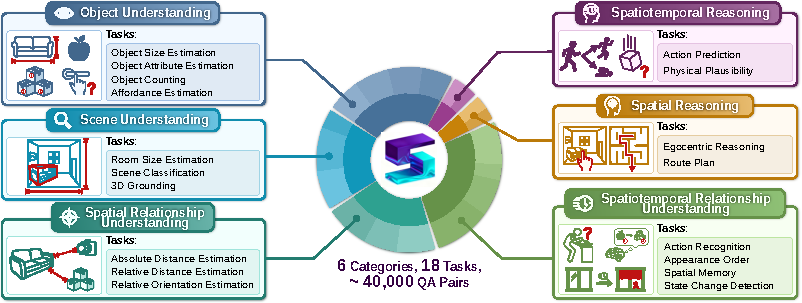
\includegraphics[width=0.99\linewidth]{Figures/overview_v2.pdf} 		
	\caption{
    An overview of Spatial4D-Bench.
    Spatial4D-Bench is a large-scale, multi-task evaluation benchmark to comprehensively assess MLLMs' 4D spatial reasoning abilities.
    It consists of \textasciitilde40,000 question-answer pairs covering 18 well-defined tasks, which are organized into 6 categories, including object understanding, scene understanding, spatial relationship understanding, spatiotemporal relationship understanding, spatial reasoning and spatiotemporal reasoning, covering various aspects of 4D spatial reasoning.
    Example question-answer pairs can be found in the appendix.
	\label{fig_spatial4dbench_overview} }
\end{figure}


\begin{table}[t]
\centering
\footnotesize
\setlength{\tabcolsep}{2.5pt} 
\begin{tabular}{llcccccccc}
\toprule
 & & & & \multicolumn{6}{c}{\textbf{Cognitive Categories}} \\
 \cmidrule(lr){5-10}
 & & \textbf{\# Eval} & \textbf{\# } & 
\multicolumn{1}{c}{\textbf{Object}} & 
\multicolumn{1}{c}{\textbf{Scene}} & 
\multicolumn{1}{c}{\textbf{Spatial}} & 
\multicolumn{1}{c}{\textbf{S.T.}} & 
\multicolumn{1}{c}{\textbf{Spatial}} & 
\multicolumn{1}{c}{\textbf{S.T.}} \\ 
\textbf{Benchmark} & \textbf{Pub.} & \textbf{QA} & \textbf{Tasks} & 
\multicolumn{1}{c}{\textbf{Und.}} & 
\multicolumn{1}{c}{\textbf{Und.}} & 
\multicolumn{1}{c}{\textbf{Rel.}} & 
\multicolumn{1}{c}{\textbf{Rel.}} & 
\multicolumn{1}{c}{\textbf{Reas.}} & 
\multicolumn{1}{c}{\textbf{Reas.}} \\ 
\midrule


SpatialRGPT~\cite{cheng2024spatialrgpt} & Jun. 2024 & 1,406 & 2 & \xmark & \xmark & \cmark & \xmark & \xmark & \xmark \\

3DSRBench~\cite{ma20243dsrbench} & Dec. 2024 & 2,772 & 4 & \textcolor{Goldenrod}{\textbf{\LEFTcircle}} & \xmark & \cmark & \xmark & \xmark & \xmark \\

VSI-Bench~\cite{Yang_2025_CVPR} & Dec. 2024 & 5,156 & 8 & \textcolor{Goldenrod}{\textbf{\LEFTcircle}} & \textcolor{Goldenrod}{\textbf{\LEFTcircle}} & \cmark & \textcolor{Goldenrod}{\textbf{\LEFTcircle}} & \textcolor{Goldenrod}{\textbf{\LEFTcircle}} & \xmark \\


STI-Bench~\cite{li2025sti} & Mar. 2025 & 2,064 & 8 & \textcolor{Goldenrod}{\textbf{\LEFTcircle}} & \textcolor{Goldenrod}{\textbf{\LEFTcircle}} & \cmark & \textcolor{Goldenrod}{\textbf{\LEFTcircle}} & \xmark & \xmark \\

LEGO-Puzzles~\cite{tang2025lego} & Mar. 2025 & 1,100 & 11 & \xmark & \xmark & \xmark & \textcolor{Goldenrod}{\textbf{\LEFTcircle}} & \xmark & \textcolor{Goldenrod}{\textbf{\LEFTcircle}} \\

MMSI-Bench~\cite{yang2025mmsi} & May. 2025 & 1,000 & 4 & \xmark & \xmark & \cmark & \textcolor{Goldenrod}{\textbf{\LEFTcircle}} & \xmark & \xmark \\

MIRAGE~\cite{liu2025mirage} & May. 2025 & 1,710 & 3 & \textcolor{Goldenrod}{\textbf{\LEFTcircle}} & \xmark & \textcolor{Goldenrod}{\textbf{\LEFTcircle}} & \textcolor{Goldenrod}{\textbf{\LEFTcircle}} & \xmark & \xmark \\

SpaCE-10~\cite{gong2025space} & Jun. 2025 & 5,000 & 8 & \textcolor{Goldenrod}{\textbf{\LEFTcircle}} & \textcolor{Goldenrod}{\textbf{\LEFTcircle}} & \cmark & \xmark & \xmark & \xmark \\

InternSpatial~\cite{deng2025internspatial} & Jun. 2025 & 6,008 & 4 & \textcolor{Goldenrod}{\textbf{\LEFTcircle}} & \xmark & \cmark & \xmark & \xmark & \xmark \\

VLM4D~\cite{zhou2025vlm4d} & Aug. 2025 & 1,816 & 4 & \xmark & \xmark & \xmark & \cmark & \xmark & \xmark \\

SIBench~\cite{yu2025far} & Sep. 2025 & 9,000 & 7 & \textcolor{Goldenrod}{\textbf{\LEFTcircle}} & \textcolor{Goldenrod}{\textbf{\LEFTcircle}} & \cmark & \textcolor{Goldenrod}{\textbf{\LEFTcircle}} & \textcolor{Goldenrod}{\textbf{\LEFTcircle}} & \textcolor{Goldenrod}{\textbf{\LEFTcircle}} \\

\midrule
\textbf{Spatial4D-Bench} & \textbf{Ours} & \textbf{39,305} & \textbf{18} & \cmark & \cmark & \cmark & \cmark & \cmark & \cmark \\ 
\midrule[0.08em]
\multicolumn{10}{c}{\cmark: fully covered\quad  \textcolor{Goldenrod}{\textbf{\LEFTcircle}}: partially covered \quad \xmark: not covered}
\end{tabular}%
\vspace{0.5em}
    \caption{Comparison of Spatial4D-Bench with state-of-the-art spatial intelligence benchmarks. We evaluate coverage across 6 cognitive categories: object understanding (size, attribute, count and affordance), scene understanding (room size, scene class and grounding), spatial relationships (absolute/relative distance and orientation), spatiotemporal (S.T.) relationships (action, order, memory and state change), spatial reasoning (egocentric and route plan), and spatiotemporal reasoning (prediction and physical plausibility). Unlike prior works, Spatial4D-Bench provides significantly higher data scale and comprehensive coverage of all 18 tasks, offering a robust evaluation of MLLMs' 4D reasoning capabilities.}
    \label{tab:recent_mllm_eval_benchmarks}
\end{table}


In this work, we present \textbf{Spatial4D-Bench}, a large-scale, multi-task 4D spatial intelligence benchmark that enables comprehensive assessment of MLLMs' spatial reasoning abilities. As shown in \cref{fig_spatial4dbench_overview}, Spatial4D-Bench comprises \textasciitilde40,000 carefully curated and annotated question-answer (QA) pairs, covering a wide variety of indoor and outdoor environments involving diverse objects, actions, and scenes.
By adhering to human spatial cognition principles~\cite{waller2013handbook, newcombe2004spatial}, these QA pairs are divided into 6 categories, namely, \textit{object understanding}, \textit{scene understanding}, \textit{spatial relationship understanding}, \textit{spatiotemporal relationship understanding}, \textit{spatial reasoning}, and \textit{spatiotemporal reasoning}.
Each category is further subdivided into various tasks, yielding 18 tasks in total that span a broad range of spatial perception, understanding and reasoning abilities.
This significantly distinguishes Spatial4D-Bench from existing benchmarks that are often small-scale or limited in diversity.
Although existing benchmarks have covered some tasks (\eg, object size estimation and object counting) overlapping with Spatial4D-Bench, some 4D tasks presented in Spatial4D-Bench remain insufficiently investigated, including but not limited to \textit{spatial memory}, \textit{state change detection}, and \textit{physical plausibility reasoning}.
Therefore, compared to existing benchmarks, Spatial4D-Bench provides a more comprehensive evaluation suite for the assessment of MLLMs' spatial cognition abilities, spanning a variety of tasks that parallel the versatility of human spatial intelligence. 
\cref{tab:recent_mllm_eval_benchmarks} summarizes the statistical differences between Spatial4D-Bench and existing benchmarks.

We conduct thorough experiments to benchmark a variety of state-of-the-art MLLMs on Spatial4D-Bench, including two proprietary MLLMs (GPT-5~\cite{OpenAI2025} and Gemini 2.5-Pro~\cite{Gemini2025}) and several open-source MLLMs (VideoLLama3~\cite{zhang2025videollama}, Qwen2.5-VL~\cite{bai2025qwen2}, Qwen3-VL~\cite{bai2025qwen2}, and InternVL3.5~\cite{wang2025internvl3}) with model sizes ranging from 7B to 241B parameters.
Our extensive experiments and in-depth analysis reveal that MLLMs still exhibit a performance gap relative to humans in comprehensive 4D spatial reasoning.
In particular, MLLMs have substantial limitations in a wide variety of 4D spatial reasoning aspects, such as route plan, egocentric reasoning, and physical plausibility reasoning.
Nevertheless, we also observe that MLLMs surpass human performance on certain tasks, such as room size and object size estimation.
This is reasonable, as humans generally struggle with tasks that require the accurate estimation of 3D scale in real world, while MLLMs can outperform humans by leveraging vast amounts of training data to provide prior knowledge.
We hope that these findings provide valuable insights to the community and that the release of Spatial4D-Bench facilitates the development of more capable MLLMs toward human-level 4D spatial intelligence.
More resources can be found on our project page: \url{https://spatial4d-bench.github.io/spatial4d/}.

